\documentclass{beamer}
\usepackage[utf8]{inputenc}

\usetheme{Madrid}
\usecolortheme{default}
\usepackage{amsmath,amssymb,amsfonts,amsthm}
\usepackage{txfonts}
\usepackage{tkz-euclide}
\usepackage{listings}
\usepackage{adjustbox}
\usepackage{array}
\usepackage{tabularx}
\usepackage{gvv}
\usepackage{lmodern}
\usepackage{circuitikz}
\usepackage{tikz}
\usepackage{graphicx}
\usepackage{mathtools}
\setbeamertemplate{page number in head/foot}[totalframenumber]

\usepackage{tcolorbox}
\tcbuselibrary{minted,breakable,xparse,skins}



\definecolor{bg}{gray}{0.95}
\DeclareTCBListing{mintedbox}{O{}m!O{}}{%
  breakable=true,
  listing engine=minted,
  listing only,
  minted language=#2,
  minted style=default,
  minted options={%
    linenos,
    gobble=0,
    breaklines=true,
    breakafter=,,
    fontsize=\small,
    numbersep=8pt,
    #1},
  boxsep=0pt,
  left skip=0pt,
  right skip=0pt,
  left=25pt,
  right=0pt,
  top=3pt,
  bottom=3pt,
  arc=5pt,
  leftrule=0pt,
  rightrule=0pt,
  bottomrule=2pt,
  toprule=2pt,
  colback=bg,
  colframe=orange!70,
  enhanced,
  overlay={%
    \begin{tcbclipinterior}
    \fill[orange!20!white] (frame.south west) rectangle ([xshift=20pt]frame.north west);
    \end{tcbclipinterior}},
  #3,
}
\lstset{
    language=C,
    basicstyle=\ttfamily\small,
    keywordstyle=\color{blue},
    stringstyle=\color{orange},
    commentstyle=\color{green!60!black},
    numbers=left,
    numberstyle=\tiny\color{gray},
    breaklines=true,
    showstringspaces=false,
}
%This block of code defines the information to appear in the
%Title page
\title %optional
{1.10.25}
%\subtitle{A short story}

\author % (optional)
{Vaishnavi - EE25BTECH11059}



\begin{document}


\frame{\titlepage}
\begin{frame}{Question}
If a line makes angles $90^\circ$, $60^\circ$, and $30^\circ$ with the positive directions of the $X$, $Y$, and $Z$ axes respectively, find its direction cosines.
 

\end{frame}
\begin{frame}{Definition}
Definition of Direction Cosines: Direction cosines are the cosine values of the angles a vector makes with the $x$, $y$, and $z$ axes; they are the components of the unit vector along $x$,$y$,$z$ axes 
\end{frame}
\begin{frame}{allowframebreaks}
\frametitle{Solution}
\begin{table}[H]    
  \centering
  \begin{tabular}{|c|c|c|c|}
\hline
Angle (\(\alpha\)) & \(\cos(\alpha)\) & Value & Axis \\
\hline
\(90^\circ\) & \(\cos(90^\circ) = 0\) & \(l = 0\) & x-axis \\
\(60^\circ\) & \(\cos(60^\circ) = \frac{1}{2}\) & \(m = \frac{1}{2}\) & y-axis \\
\(30^\circ\) & \(\cos(30^\circ) = \frac{\sqrt{3}}{2}\) & \(n = \frac{\sqrt{3}}{2}\) & z-axis \\
\hline
\end{tabular}
  \caption{Variables Used}
  \label{tab:1.10.25}
\end{table}

\end{frame}


\begin{frame}{Solution}
Let the direction cosines be 
$l$,$m$,$n$\\
$l$,$m$,$n$, which are the cosines of the angles that the line makes with the $X$, $Y$, and $Z$ axes respectively.\\
\begin{align}
      l = \cos(90^\circ) = 0  \\
      m = \cos(60^\circ) = \frac{1}{2} \\
      n = \cos(30^\circ) = \frac{\sqrt{3}}{2}  
\end{align}
      
      A key property is that the sum of the squares of the direction cosines always equals one:  $l^2 + m^2 + n^2 = 1 $
\end{frame}

\begin{frame}{solution}
\begin{align}
    \text{unit vector in direction of} \vec{x}= \myvec{
                                                0
                                                \\
                                                 \frac{1}{2}
                                                  \\
                                                  \frac{\sqrt{3}}{2}
                                                  }
\end{align}
\end{frame}
\begin{frame}{Graph}
   Refer to Figure

\begin{figure}[H]
\begin{center}
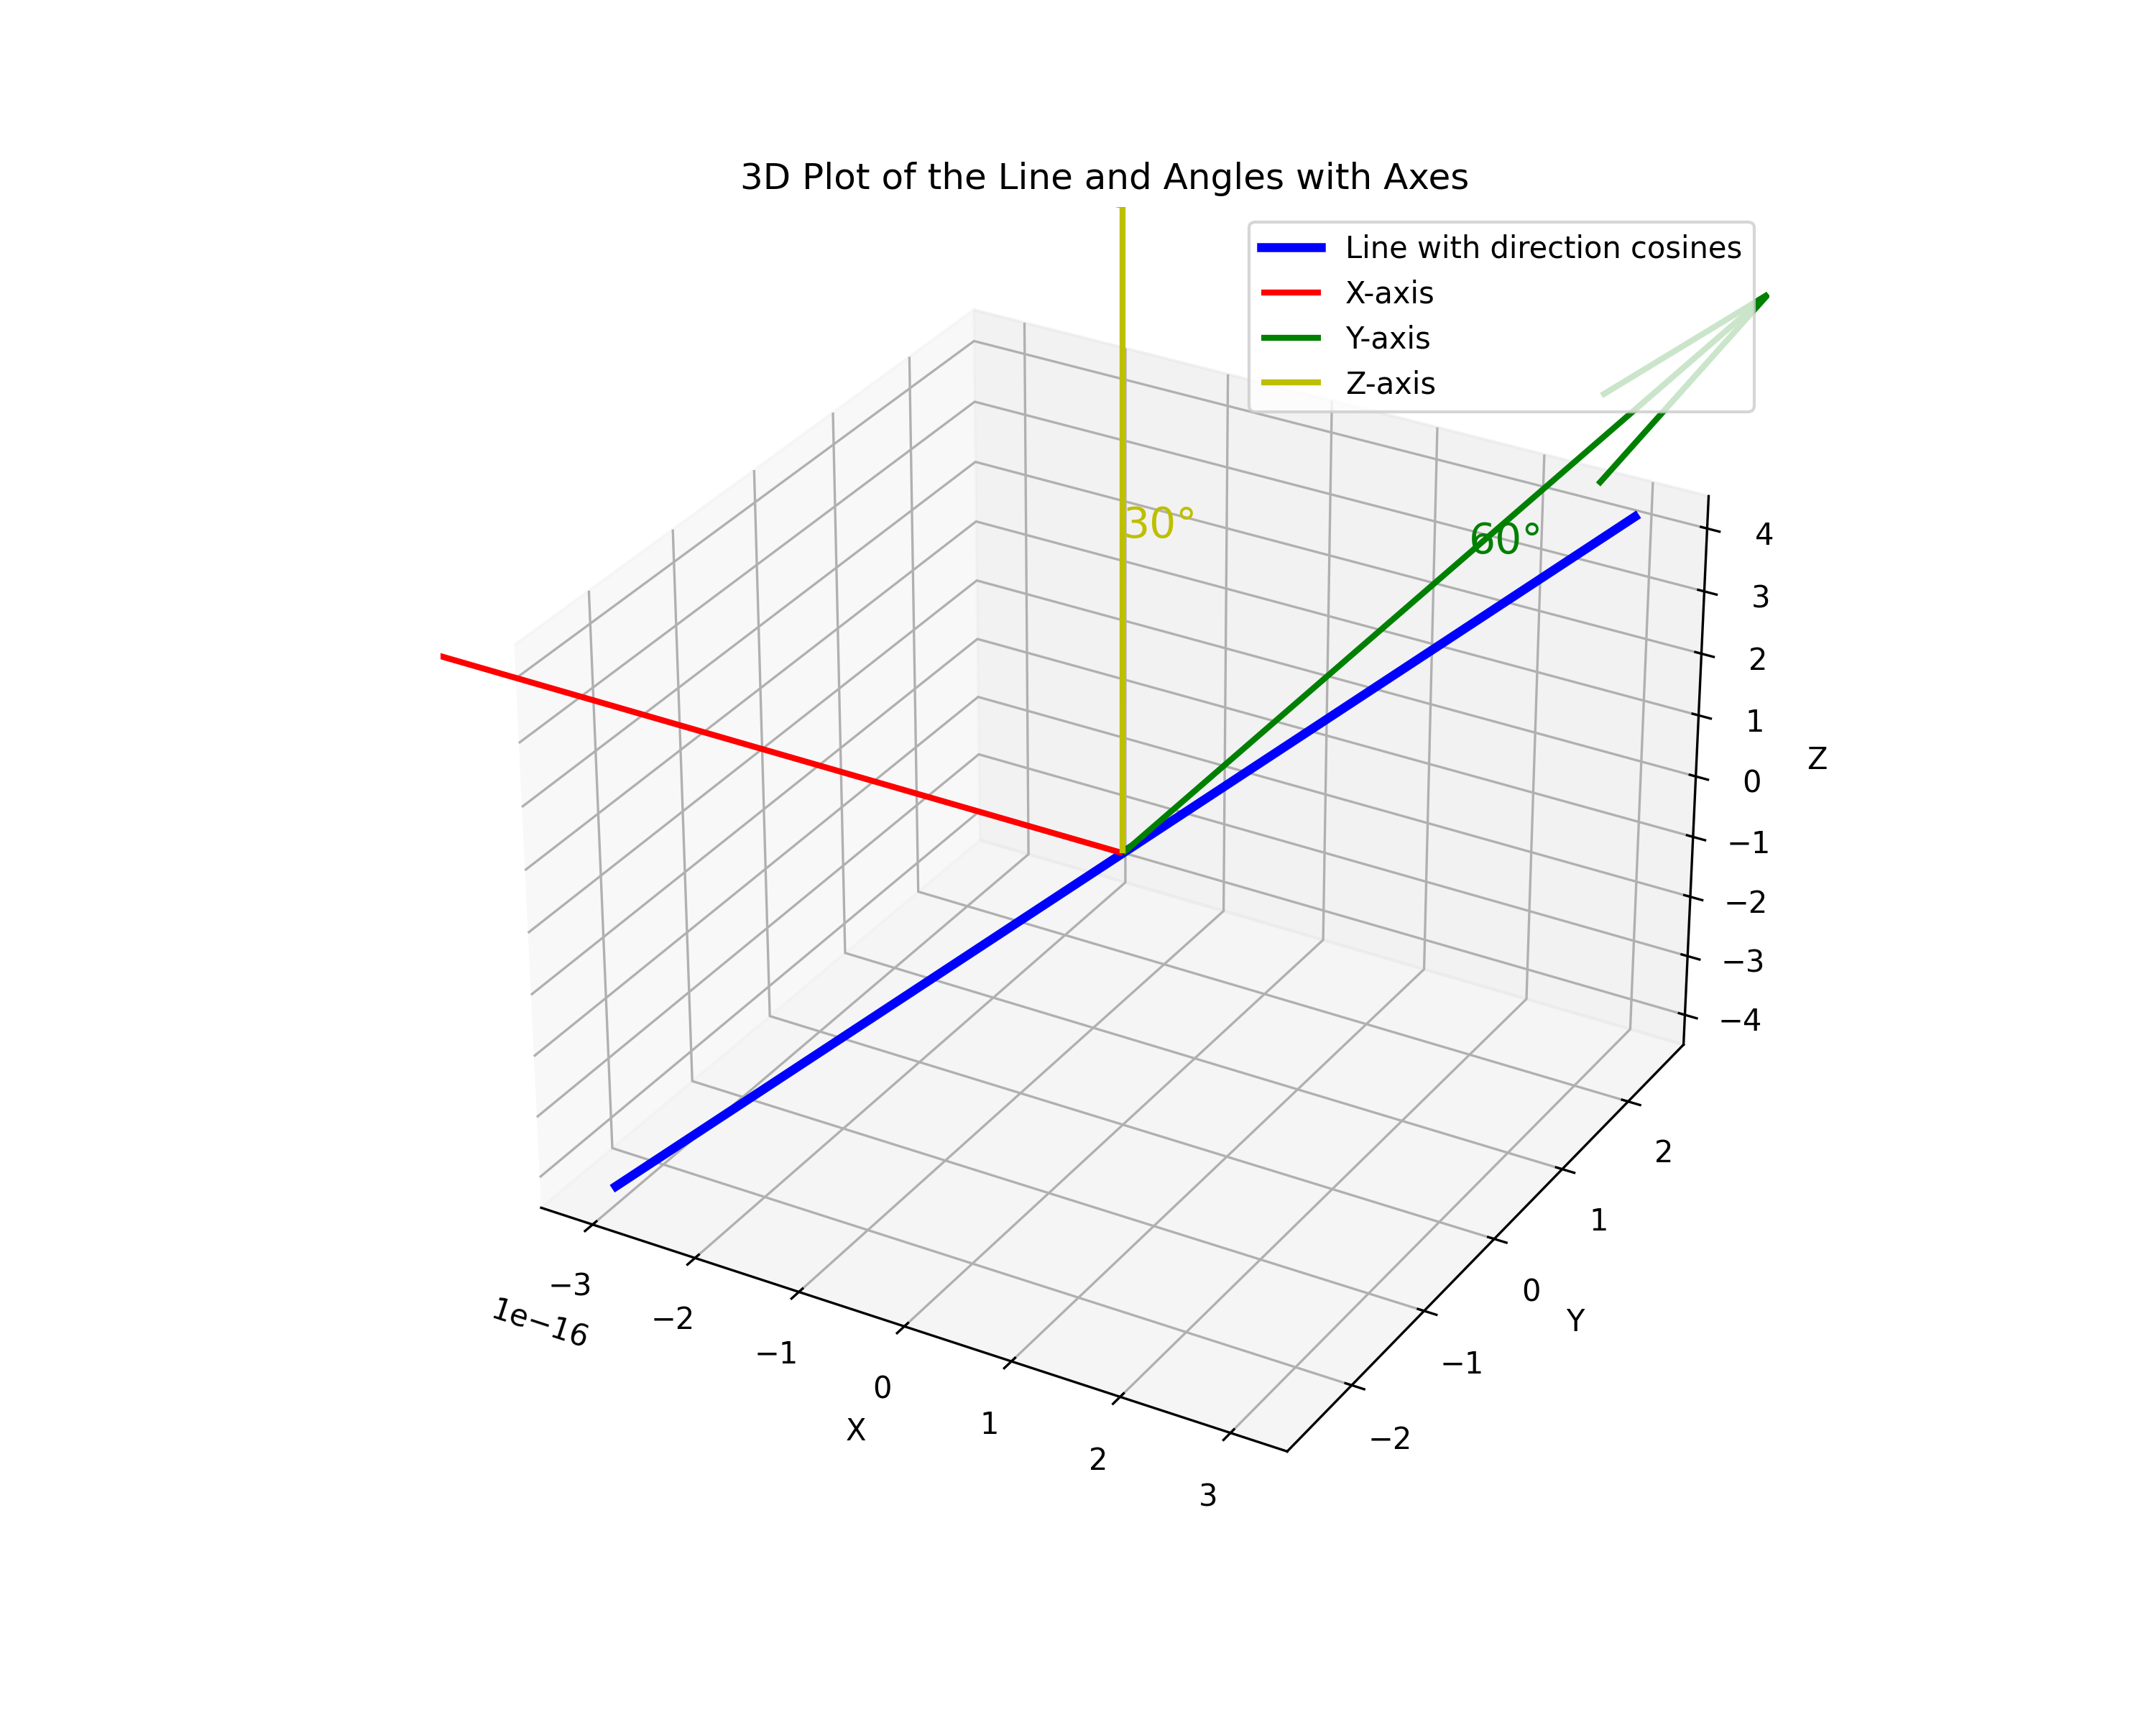
\includegraphics[width=0.6\columnwidth]{../figs/graph2.png}
\end{center}
\caption{}
\label{fig:Fig}
\end{figure}  
\end{frame}



\begin{frame}[fragile]
    \frametitle{Python Code}
    \begin{lstlisting}
 import numpy as np
import matplotlib.pyplot as plt
from mpl_toolkits.mplot3d import Axes3D

# Create a figure and 3D axis
fig = plt.figure()
ax = fig.add_subplot(111, projection='3d')

# Define the line with direction cosines
x = np.linspace(-3, 3, 100)
y = np.linspace(-3, 3, 100)
z = np.linspace(-3, 3, 100)

# Direction cosines for the line (example: cosines of 30°, 60°)
cos_30 = np.cos(np.radians(30))
cos_60 = np.cos(np.radians(60))


\end{lstlisting}
\end{frame}

\begin{frame}[fragile]
    \frametitle{Python Code}

    \begin{lstlisting}
# Parametric equations for the line with direction cosines
x_line = x * cos_30
y_line = y * cos_60
z_line = z
# Plot the line
ax.plot(x_line, y_line, z_line, label='Line with direction cosines', color='b')

# Plot the axes (X, Y, Z)
ax.plot([0, 3], [0, 0], [0, 0], color='r', label='X-axis')
ax.plot([0, 0], [0, 3], [0, 0], color='g', label='Y-axis')
ax.plot([0, 0], [0, 0], [0, 3], color='y', label='Z-axis')




    \end{lstlisting}
\end{frame}

\begin{frame}[fragile]
    \frametitle{Python Code}

    \begin{lstlisting}
 # Set labels
ax.set_xlabel('X')
ax.set_ylabel('Y')
ax.set_zlabel('Z')

# Set the title
ax.set_title('3D Plot of the Line and Angles with Axes')

# Display the legend
ax.legend()
# Save the figure
fig.savefig("collinear_3d_plot.png")

# Show the plot
plt.show()




    \end{lstlisting}
\end{frame}

\begin{frame}[fragile]
\frametitle{C Code}
\begin{lstlisting}
#include <stdio.h>
#include <math.h>

#define DEG_TO_RAD(deg) ((deg) * (M_PI / 180.0))

int main() {
    // Define the angles in degrees
    double alpha = 90.0;  // Angle with X-axis
    double beta = 60.0;   // Angle with Y-axis
    double gamma = 30.0;  // Angle with Z-axis
    
    // Convert degrees to radians
    double alpha_rad = DEG_TO_RAD(alpha);
    double beta_rad = DEG_TO_RAD(beta);
    double gamma_rad = DEG_TO_RAD(gamma);

    \end{lstlisting}

\end{frame}

\begin{frame}[fragile]
\frametitle{C Code}
\begin{lstlisting}
    // Calculate the direction cosines
    double l = cos(alpha_rad);  // cos(90 degrees)
    double m = cos(beta_rad);   // cos(60 degrees)
    double n = cos(gamma_rad);  // cos(30 degrees)

    // Print the direction cosines
    printf("Direction Cosines of the vector:\n");
    printf("l = cos(90 degrees) = %.2f\n", l);
    printf("m = cos(60 degrees) = %.2f\n", m);
    printf("n = cos(30 degrees) = %.2f\n", n);

    // Display the vector (l, m, n)
    printf("Direction cosines of vector x = (%.2f, %.2f, %.2f)\n", l, m, n);

    return 0;
}
\end{lstlisting}
\end{frame}


\begin{frame}[fragile]
\frametitle{Python and C Code}

\begin{lstlisting}
import subprocess

# Compile the C program
subprocess.run(["gcc", "points.c", "-o", "points"])

# Run the compiled C program
result = subprocess.run(["./points"], capture_output=True, text=True)

# Print the output from the C program (direction cosines)
print(result.stdout) 

\end{lstlisting}

\end{frame}

 





\end{document}